% Options for packages loaded elsewhere
\PassOptionsToPackage{unicode}{hyperref}
\PassOptionsToPackage{hyphens}{url}
%
\documentclass[
  english,
]{book}
\usepackage{amsmath,amssymb}
\usepackage{lmodern}
\usepackage{ifxetex,ifluatex}
\ifnum 0\ifxetex 1\fi\ifluatex 1\fi=0 % if pdftex
  \usepackage[T1]{fontenc}
  \usepackage[utf8]{inputenc}
  \usepackage{textcomp} % provide euro and other symbols
\else % if luatex or xetex
  \usepackage{unicode-math}
  \defaultfontfeatures{Scale=MatchLowercase}
  \defaultfontfeatures[\rmfamily]{Ligatures=TeX,Scale=1}
\fi
% Use upquote if available, for straight quotes in verbatim environments
\IfFileExists{upquote.sty}{\usepackage{upquote}}{}
\IfFileExists{microtype.sty}{% use microtype if available
  \usepackage[]{microtype}
  \UseMicrotypeSet[protrusion]{basicmath} % disable protrusion for tt fonts
}{}
\makeatletter
\@ifundefined{KOMAClassName}{% if non-KOMA class
  \IfFileExists{parskip.sty}{%
    \usepackage{parskip}
  }{% else
    \setlength{\parindent}{0pt}
    \setlength{\parskip}{6pt plus 2pt minus 1pt}}
}{% if KOMA class
  \KOMAoptions{parskip=half}}
\makeatother
\usepackage{xcolor}
\IfFileExists{xurl.sty}{\usepackage{xurl}}{} % add URL line breaks if available
\IfFileExists{bookmark.sty}{\usepackage{bookmark}}{\usepackage{hyperref}}
\hypersetup{
  pdftitle={DRAFT: ReCentering Psych Stats: Multivariate Modeling},
  pdfauthor={Lynette H Bikos, PhD, ABPP},
  pdflang={en},
  hidelinks,
  pdfcreator={LaTeX via pandoc}}
\urlstyle{same} % disable monospaced font for URLs
\usepackage{longtable,booktabs,array}
\usepackage{calc} % for calculating minipage widths
% Correct order of tables after \paragraph or \subparagraph
\usepackage{etoolbox}
\makeatletter
\patchcmd\longtable{\par}{\if@noskipsec\mbox{}\fi\par}{}{}
\makeatother
% Allow footnotes in longtable head/foot
\IfFileExists{footnotehyper.sty}{\usepackage{footnotehyper}}{\usepackage{footnote}}
\makesavenoteenv{longtable}
\usepackage{graphicx}
\makeatletter
\def\maxwidth{\ifdim\Gin@nat@width>\linewidth\linewidth\else\Gin@nat@width\fi}
\def\maxheight{\ifdim\Gin@nat@height>\textheight\textheight\else\Gin@nat@height\fi}
\makeatother
% Scale images if necessary, so that they will not overflow the page
% margins by default, and it is still possible to overwrite the defaults
% using explicit options in \includegraphics[width, height, ...]{}
\setkeys{Gin}{width=\maxwidth,height=\maxheight,keepaspectratio}
% Set default figure placement to htbp
\makeatletter
\def\fps@figure{htbp}
\makeatother
\setlength{\emergencystretch}{3em} % prevent overfull lines
\providecommand{\tightlist}{%
  \setlength{\itemsep}{0pt}\setlength{\parskip}{0pt}}
\setcounter{secnumdepth}{5}
\usepackage{booktabs}
\ifxetex
  % Load polyglossia as late as possible: uses bidi with RTL langages (e.g. Hebrew, Arabic)
  \usepackage{polyglossia}
  \setmainlanguage[]{english}
\else
  \usepackage[main=english]{babel}
% get rid of language-specific shorthands (see #6817):
\let\LanguageShortHands\languageshorthands
\def\languageshorthands#1{}
\fi
\ifluatex
  \usepackage{selnolig}  % disable illegal ligatures
\fi
\usepackage[]{natbib}
\bibliographystyle{plainnat}

\title{DRAFT: ReCentering Psych Stats: Multivariate Modeling}
\author{Lynette H Bikos, PhD, ABPP}
\date{}

\begin{document}
\maketitle

{
\setcounter{tocdepth}{1}
\tableofcontents
}
\hypertarget{preface}{%
\chapter*{Preface}\label{preface}}
\addcontentsline{toc}{chapter}{Preface}

\textbf{If you are viewing this document, you should know that this is a book-in-progress. Early drafts are released for the purpose teaching my classes and gaining formative feedback from a host of stakeholders. The document was last updated on 15 Mar 2021}

To \emph{center} a variable in regression means to set its value at zero and interpret all other values in relation to this reference point. Regarding race and gender, researchers often center male and White at zero. Further, it is typical that research vignettes in statistics textbooks are similarly seated in a White, Western (frequently U.S.), heteronormative, framework. The purpose of this project is to create a set of open educational resources (OER) appropriate for doctoral and post-doctoral training that contribute to justice, equity, diversity, inclusion (JEDI), and social responsivity.

Statistics training in doctoral programs are frequently taught with fee-for-use programs (e.g., SPSS/AMOS, SAS, MPlus) that may not be readily available to the post-doctoral professional. In recent years, there has been an increase and improvement in R packages (e.g., \emph{psych}, \emph{lavaan}) used for in analyses common to psychological research. Correspondingly, many graduate programs are transitioning to statistics training in R (free and open source). This is a challenge for post-doctoral psychologists who were trained with other software. This OER will offer statistics training with R and be, freely available on open science platforms under a Creative Commons Attribution - Non Commercial - Share Alike license {[}CC BY-NC-SA 4.0{]}.

Training models for doctoral programs in HSP are commonly scholar-practitioner, scientist-practitioner, or clinical-scientist. An emerging model, the \emph{scientist-practitioner-advocacy} training model incorporates social justice advocacy so that graduates are equipped to recognize and address the sociocultural context of oppression and unjust distribution of resources and opportunities \citep{mallinckrodt_scientist-practitioner-advocate_2014}. In statistics textbooks, the use of research vignettes engages the learner around a tangible scenario for identifying independent variables, dependent variables, covariates, and potential mechanisms of change. Many students recall examples in Field's \citeyearpar{field_discovering_2012} popular statistics text: Viagra to teach one-way ANOVA, beer goggles for two-way ANOVA, and bushtucker for repeated measures. What if the research vignettes were investigations around JEDI/social responsivity and highlighted the scholarship of individuals whose identities are often marginalized?

In this OER, research vignettes will be from recently published articles where: (a) the author's identity is from a group where scholarship is historically marginalized (e.g., BIPOC, LGBTQ+, emerging nations), (b) the research has a JEDI/social responsivity focus, (b) the lesson's statistic is used in the article, and (c) the data is shared publicly or there is sufficient information in the article to simulate the data for the chapter example(s) and practice problem(s).

\begin{figure}
\centering
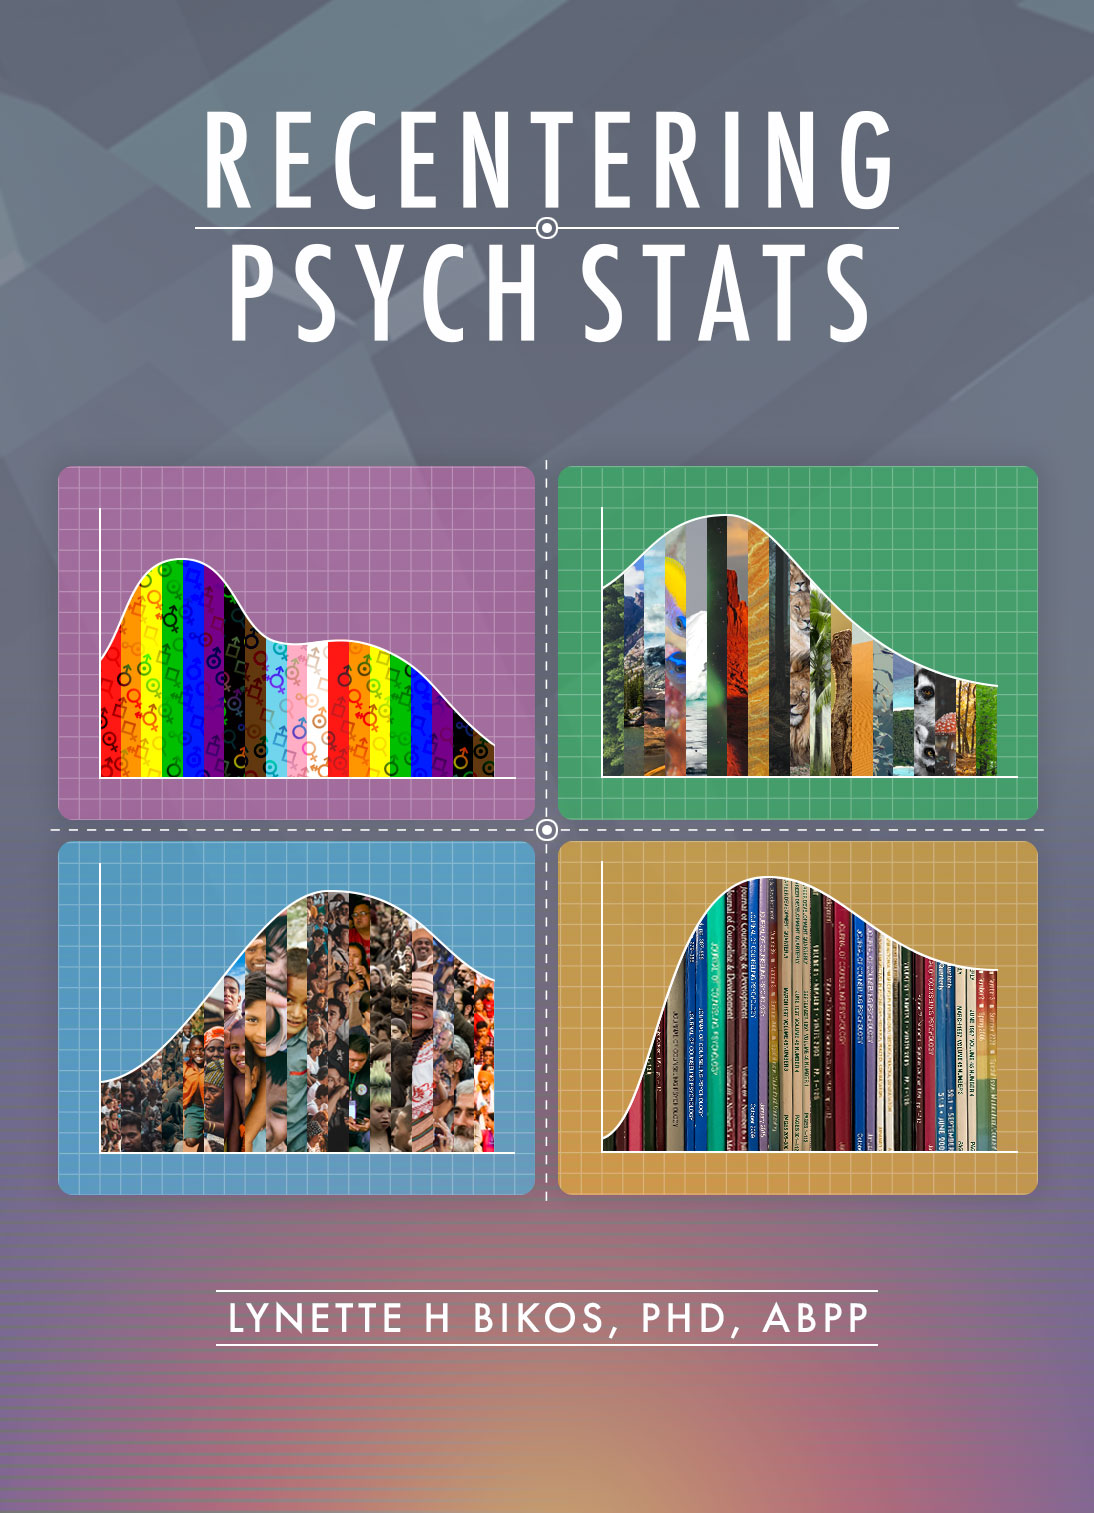
\includegraphics{ReCenter_bookcover.jpg}
\caption{An image of the book cover. It includes four quadrants of non-normal distributions representing gender, race/ethnicty, sustainability/global concerns, and journal articles}
\end{figure}

\hypertarget{copyright-with-open-access}{%
\section*{Copyright with Open Access}\label{copyright-with-open-access}}
\addcontentsline{toc}{section}{Copyright with Open Access}

This book is published under a a Creative Commons Attribution-NonCommercial-ShareAlike 4.0 International License. This means that this book can be reused, remixed, retained, revised and redistributed (including commercially) as long as appropriate credit is given to the authors. If you remix, or modify the original version of this open textbook, you must redistribute all versions of this open textbook under the same license - CC BY-SA.

Our GitHub open-source repository contains all of the text and source code for the book, including data and images.

\hypertarget{ReCintro}{%
\chapter{INTRODUCTION}\label{ReCintro}}

\hypertarget{what-to-expect-in-each-chapter}{%
\section{What to expect in each chapter}\label{what-to-expect-in-each-chapter}}

This textbook is intended as \emph{applied,} in that a primary goal is to help the scientist-practitioner-advocate use the statistic in a research problem and \emph{write it up} for a program evaluation, dissertation, or journal article. In support of that goal, I try to provide \emph{just enough} conceptual information so that the researcher can select the appropriate statistic (i.e., distinguishing between when ANOVA is appropriate and when regression is appropriate) and assign variables to their proper role (e.g., covariate, moderator, mediator).

This conceptual approach does include step-by-step \emph{hand-calculations} (only we calculate them arithmetically in R) to provide a \emph{visceral feeling} of what is happening within the statistical algorithm that may be invisible to the researcher. Additionally, the conceptual review includes a review of the assumptions about the characteristics of the data and research design that are required for the statistic. Statistics can be daunting, so I have worked hard to establish a \emph{workflow} through each analysis. When possible, I include a flowchart that is referenced frequently in each chapter and assists the the researcher keep track of their place in the many steps and choices that accompany even the simplest of analyses.

As with many statistics texts, each chapter includes a \emph{research vignette.} Somewhat unique to this resource is that the vignettes are selected from recently published articles. Each vignette is chosen with the intent to meet as many of the following criteria as possible:

\begin{itemize}
\tightlist
\item
  the statistic that is the focus of the chapter was properly used in the article,
\item
  the author's identity is from a group where scholarship is historically marginalized (e.g., BIPOC, LGBTQ+, emerging nations),
\item
  the research has a justice, equity, inclusion, diversity, and social responsivity focus and will contribute positively to a social justice pedagogy, and
\item
  the data is available in a repository or there is sufficient information in the article to simulate the data for the chapter example(s) and practice problem(s).
\end{itemize}

In each chapter we employ \emph{R} packages that will efficiently calculate the statistic and the dashboard of metrics (e.g., effect sizes, confidence intervals) that are typically reported in psychological science.

\hypertarget{if-you-are-new-to-r}{%
\section{If You are New to R}\label{if-you-are-new-to-r}}

In this section I will provide some orientation to using R in psychological research. I don't intend this text to be ``R from the ground up,'' but I will provide enough guidance that the individual can start working the problems.

I will also link to tutorials that help individuals get started in R.

\hypertarget{r-hygiene}{%
\subsection{R Hygiene}\label{r-hygiene}}

Many problems in R can be resolved with good ``R hygiene.'' I will review those practices here. I will also review the conventions I will try to consistently use throughout the text.

Everything in a folder

Although it is often considered good R etiquette to load all packages at the beginning of the script, this is not my practice. Each chapter will include a script that lists all the packages used, but I will open each package as we use it. This will provide a greater sense of which packages are needed for what task.

\hypertarget{maximizing-learning-by-accessing-all-the-resources}{%
\section{Maximizing Learning by Accessing all the Resources}\label{maximizing-learning-by-accessing-all-the-resources}}

In this section I will talk about the options for using and learning the materials. Primarily these are:

\begin{enumerate}
\def\labelenumi{\arabic{enumi}.}
\tightlist
\item
  Open a new document of R, copying the script over and running it in a fresh document.
\item
  Forking the entire suite of materials from GitHub and working directly in the original R markdown documents with the option to annotate the material directly.
\item
  Forking the materials to adopt and or adapt for teaching.
\item
  Listening to the accompanying lectures (I sound best when the speed is 1.75). I intend to record the lectures in Panopto which provides some closed captioning options.
\item
  Making use of the practice problems.
\end{enumerate}

  \bibliography{STATSnMETH.bib}

\end{document}
